\chapter{Operaciones cuánticas} \label{ch2}
% Intro {{{
% \janote{\h{Hey Carlos.} Dejé los comentarios del esqueleto
% del capítulo para que recordaras lo que habíamos acordado.
% Intenté dar suficiente detalle para este capítulo para introducir
% las operaciones cuánticas, pero toma en cuenta que muchas cosas
% (demostraciones, detalles más formales) los deje por fuera pensando 
% que se pueden guardar para la tesis. Mi objetivo fue conectar 
% todo el capítulo motivado en ejemplos, que a mi parecer cumple
% con el objetivo de este trabajo.
% \newline}
% \janote{
% - Introducción hablando de que las operaciones cuánticas sirven 
% para describir la dinámica de los sistemas abiertos y una guía al 
% lector de qué se viene en este cap. Enfatizar en que el truco es 
% considerar como 'nuevo sistema cerrado' al sistema extendido}
% \cpnote{No entiendo esa frase}
% \janote{Me refiero a que un sistema que interactúa con su entorno es abierto, 
% pero si consideramos al sistema total (principal+entorno) ese es cerrado.
% \textbf{Ahora que lo expliqué ya no encuentro sentido para hablar de esto aquí,
% mejor lo voy a quitar}}

Las operación cuánticas son un marco teórico que proporcionan
una manera de describir el cambio dinámico de los estados 
de los sistemas cuánticos abiertos \cite{bengtsson_zyczkowski_2017}. 
En la naturaleza es imposible
encontrar un sistema cuántico perfectamente cerrado, es decir, un 
sistema cuántico ideal que no sufra de interacción con su entorno
\cite{nielsen_chuang_2011}. Los sistemas cuánticos reales 
interaccionan con su entorno y, peor aún, en el laboratorio 
los grados de libertad del entorno son, en general, inaccesibles.
Las operaciones cuánticas son un formalismo que consideran
la naturaleza abierta de los sistemas cuánticos reales y proporciona
las herramientas para describir de manera discreta la dinámica
de este tipo de sistemas.

En la sección 2.1 vamos a discutir la condición
que deben satisfacer las operaciones cuánticas para que éstas
transformen estados entrelazados (que son positivos)
en estados positivos.
\cpnote{mejor diría algo de lo qe se pueda agarrar el lector. Algo asi 
como ``obtendremos las condiciones matemáticas necesarias para definir un 
canal válido'' o algo asi, porque si no el que no sepa, va a quedar confundido} 
\janote{Mejor?}
Vamos a motivar la definición de esta condición
a partir de un ejemplo de una operación que deforma la esfera de
Bloch de 1 qubit a un disco. Las secciones 2.2 y 2.3 introducen dos 
representaciones distintas de las operaciones cuánticas,
vamos a mostrar la conexión entre ambas representaciones
mediante la matriz de Choi de una operación cuántica. Para 
concluir, en la sección 2.4 se ilustran tres ejemplos de 
operaciones cuánticas de 1 qubit que proporcionarán familiaridad
e intuición sobre los canales cuánticos. 
% }}}
\section{Mapeos completamente positivos} % {{{
% \janote{
% Introducir la transformación de la matriz de densidad $\rho$ y hablar
% de que $\E$ transforma estados en estados.\newline}
% \janote{
%     - Motivación de la CP. Ejemplo del mapeo que deforma la esfera de Bloch
%     en un disco: presentar que el mapeo extendido para 2 qubits
%     aplicado al estado máximamente entrelazado resulta en una matriz 
%     no positiva (algo que no es estado).\newline}
% \janote{- Definición de CP del Geometry of Quantum States.\newline}
% \janote{- Concluir con que las operaciones que estudiamos deben ser CPTP.
% \newline}
En el formalismo de las operaciones cuánticas, un estado cuántico,
que está descrito por su operador de densidad $\rho$,
se transforma según la ecuación 
\begin{align}
\rho' = \E (\rho)
\label{eq:E(rho)},
\end{align} 
donde $\E$ es una operación cuántica que representa alguna evolución 
física y $\rho'$ es el estado que resulta de la evolución 
\cite{nielsen_chuang_2011}. 
\cpnote{Normalmente 
uno cita al final de la frase, a menos que no se entienda. En este caso y casi
siempre, funciona ponerla al final}
\janote{De acuerdo.}
En el capítulo anterior  establecimos 
dos ejemplos de operaciones cuánticas: la evolución unitaria 
y la medición del estado de un sistema, 
para los cuales $\E \qty(\rho)=U\rho U^{\dagger}$ y 
$\E(\rho)=\sum_mM\rho M^{\dagger}$\cpnote{Aca tienes un posible problema, porque 
entonecs no conservas la traza. Quizá yo quitaria ese ejemplo, o
pondría una suma mejor hablemos}\janote{Cierto. Si no, no 
se conserva la traza unitaria. Pondré la suma}, respectivamente. 
Una operación cuántica describe discretamente 
el cambio dinámico que un estado cuántico 
atraviesa durante un proceso físico. 

Una operación cuántica $\E$ es
una transformación lineal que mapea matrices de densidad en matrices 
de densidad \cite{bengtsson_zyczkowski_2017}. Surge entonces la siguiente
pregunta: si $\E$ es un mapeo afín de matrices de densidad, ¿es eso
suficiente para afirmar que $\E$ representa una operación física? 
La respuesta es que no, y el resto de esta sección está dedicada
explicar porqué y motivar la definición de completa positividad.  
Para que $\E$ sea una evolución física la operación debe de cumplir con dos
condiciones: (1) ser un mapeo afín de matrices de densidad, 
y (2) satisfacer una condición más fuerte que la de positividad. 

La necesidad de satisfacer esta segunda condición
es una consecuencia de la interacción que un sistema podría tener
con su entorno, un sistema secundario que vamos 
a considerar inaccesible durante el resto del capítulo.
A continuación vamos a considerar una operación 
que actúa sobre los estados de un sistema de
1 qubit y, al considerar la extensión de la misma operación
sobre un sistema de 2 qubits que se encuentra en
el estado máximamente entrelazado,
obtendremos como resultado un estado no físico.
De esa manera, se justificará la necesidad de imponer 
una condición más robusta que la de la positividad 
de las operaciones cuánticas, para exigir 
que una operación cuántica transforme estados 
positivos en estados positivos, para cualquier
extensión dimensional arbitraria del espacio
de estados del sistema.

Antes de entrar de lleno con la operación que vamos 
a considerar necesitamos establecer la forma en la 
cual representar a la matriz de densidad. La base
que vamos a utilizar serán los productos tensoriales de
las matrices de Pauli: $\{ \sigma_0, \sigma_1, \sigma_2, \sigma_3\}$,
con $\sigma_0=\1$. De esa manera, las matrices de 
densidad de 1 qubit y 2 qubits se escriben, 
respectivamente, como~\cite{nielsen_chuang_2011}
\begin{align}
\rho^1&=\frac{1}{2}\sum_{i=0}^{3} r_i\sigma_i,
& 
\rho^2&=\frac{1}{4}\sum _{i,j=0, }^{3}r_{ij}\sigma_i\otimes\sigma_j,
\label{eq:DM-1q}
\end{align}
donde $r_0=r_{00}=1$, para que se cumpla que $\Tr\qty(\rho)=1.$
Las componentes $r_i$ y $r_{ij}$ definen un vector de 4 entradas
y una matriz de $4\times4$, respectivamente. 
Para el caso de 1 qubit, el vector $\qty(r_1, r_2, r_3)$ define 
las coordenadas de un punto sobre una esfera unitaria conocida
como la esfera de Bloch.
Así, todos los estados de 1 qubit se asocian con un punto en la
esfera de Bloch. En el panel izquierdo de la 
\Fref{fig:qtm-op-motivation} se muestra la esfera de Bloch
y algunos estados de 1 qubit; los estados puros se corresponden
con puntos en la superficie de la esfera y los estados mixtos 
con puntos en el interior, incluyendo al origen.

Ahora, consideremos la operación $\E_z$ que deforma la bola de Bloch a un 
disco sobre el plano $xy$, como se muestra en la \Fref{fig:qtm-op-motivation}. 
La acción de la operación $\E_z$ sobre una matriz de densidad
de 1 qubit 
de la forma \eqref{eq:DM-1q} es equivalente a 
transformar al vector $\vec{r}$ como 
$\qty(1,r_1,r_2,r_3)\mapsto\qty(1,r_1,r_2,0)$,
notando que los subíndices $1,2,3$ se utilizan para
etiquetar a las coordenadas $x,y,z$. 
Es decir, $\E_z$ borra la componente $z$ del estado de un 1 qubit.
La matriz $\E_z\qty(\rho^1)$ es también una matriz de densidad, 
por lo cual se concluye que $\E_z$ transforma estados 
positivos en estados positivos.

\begin{figure}% {{{
\centering
\begin{minipage}{.4\textwidth}
\centering
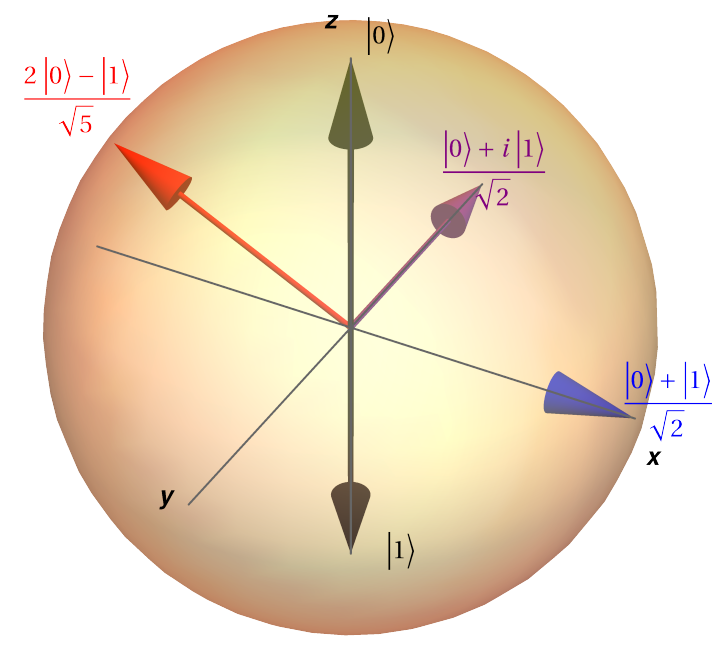
\includegraphics[width=5cm]
{img-congreso/bloch.png}
\end{minipage}
$\stackrel{\E_{z}\otimes\1 \vspace{1cm}}{\longmapsto}$
\begin{minipage}{0.4\textwidth}
\centering
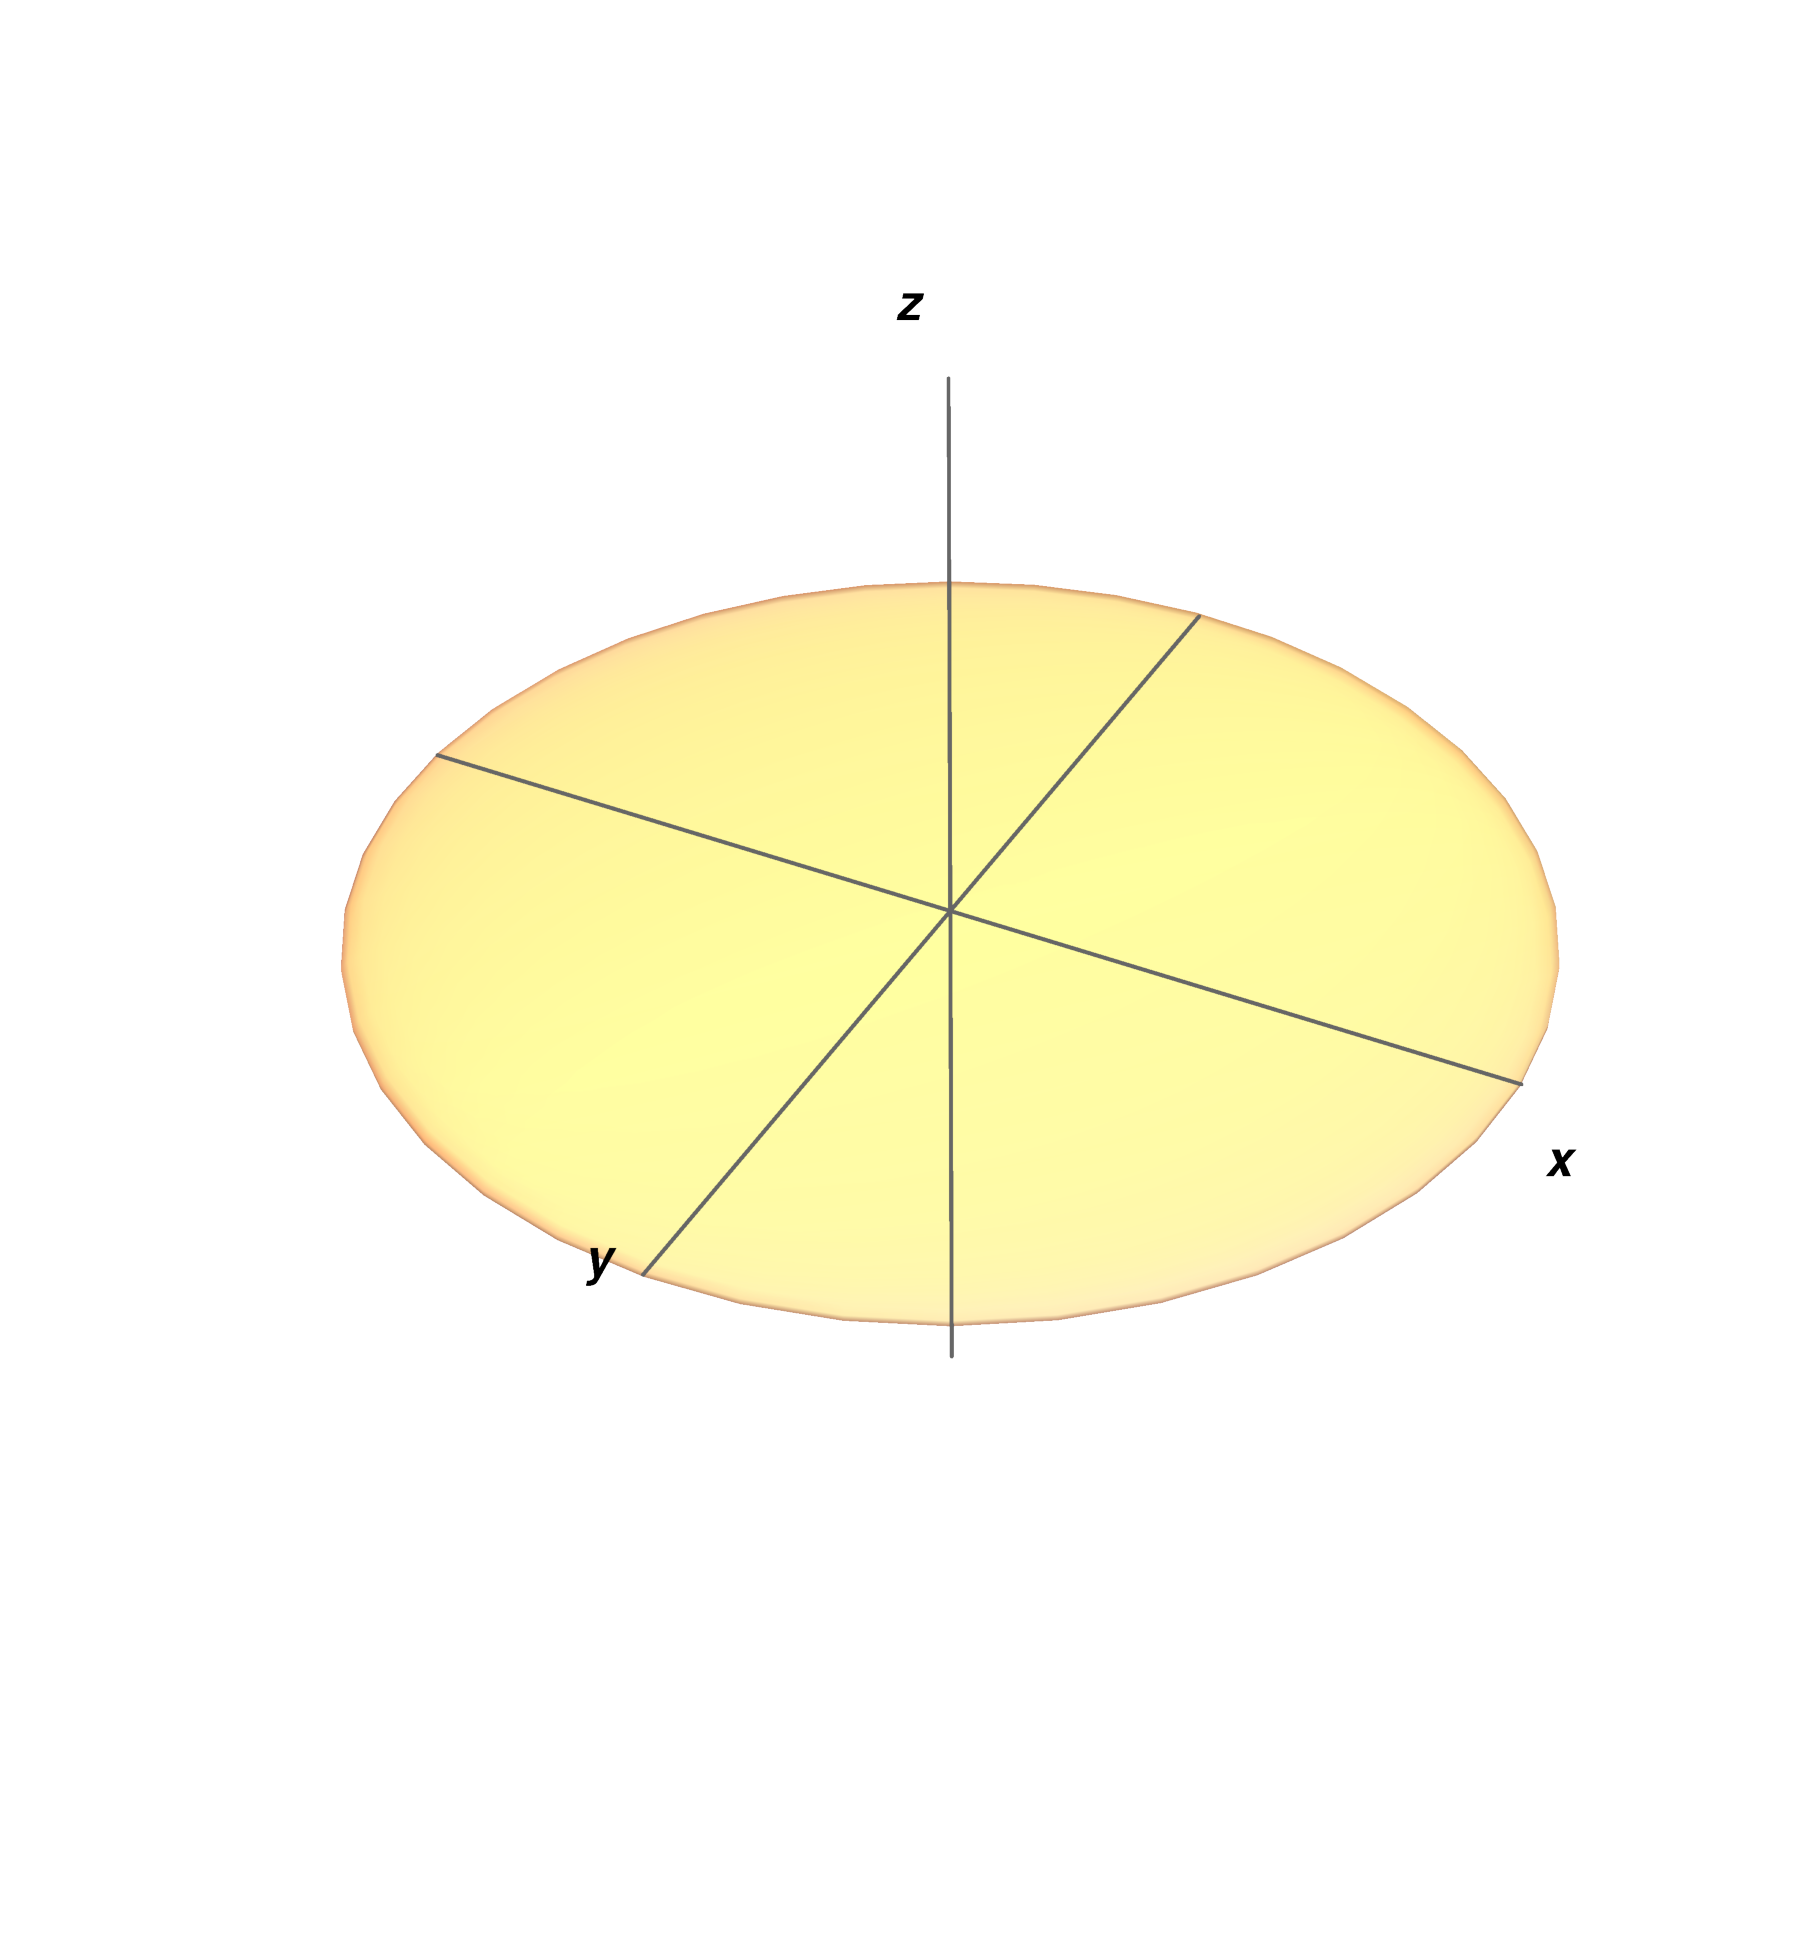
\includegraphics[width=6cm]
{img-congreso/DiskXY}
\end{minipage}
\caption{
\cpnote{Prefiero dejar a las figuras realmente flotantes}
\janote{De acuerdo}
Deformación de la esfera de Bloch a un disco sobre el plano $XY$.}
\label{fig:qtm-op-motivation}
\end{figure} % }}}

No obstante, si ahora consideramos la operación $\E_z\otimes\1$ sobre el espacio extendido
de  un sistema de 2 qubits, que se encuentra en el estado máximamente
entrelazado $\ket{\phi}=\qty(\ket{0}+\ket{1})/\sqrt{2}$, veremos 
que $\E_z\otimes\1\qty(\dyad{\phi}{\phi})$  no es una matriz de densidad.
La acción de $\E_z\otimes\1$ es tal que borra la componente
$z$ local del qubit 1 y deja intacto al resto del estado total, por consiguiente,
si la matriz de densidad es de la forma de \eqref{eq:DM-1q} entonces 
$\E_z\otimes\1$ borra las componentes $r_{3j}$ y deja invariantes 
al resto. Para calcular $\E_z\otimes\1\qty(\dyad{\phi}{\phi})$
necesitamos entonces escribir $\dyad{\phi}{\phi}$ en la base
de productos tensoriales de las matrices de Pauli.
Calculando $\dyad{\phi}{\phi}$ se tiene
\begin{align}
\dyad{\phi}{\phi}=& 
%\mqty( 
%\frac{1}{2} & 0 & 0 & \frac{1}{2} \\
%0 & 0 & 0 & 0 \\
%0 & 0 & 0 & 0 \\
%\frac{1}{2} & 0 & 0 & \frac{1}{2} \\
%)\\
%&= 
\frac{1}{2}
\Big( \dyad{00}{00} + \dyad{00}{11}
+ \dyad{11}{00} + \dyad{11}{11} \Big).
\label{eq:DM-2q-MaxE}
\end{align}
Para calcular las componentes $r_{ij}$ se calculan las
proyecciones de $\dyad{\phi}{\phi}$ sobre
los elementos $\sigma_i\otimes\sigma_j$, usando el producto interno
de Hilbert-Schmidt $\Tr\qty(\pauli{i}{j}\dyad{\phi}{\phi})$.
De esa manera, se encuentra que $r_{00}=r_{11}=r_{33}=1$, $r_{22}=-1$,
y el resto de los elementos de $r$ son iguales a cero. 
Por lo tanto, el estado máximamente entrelazado de
dos qubits, en la forma de \eqref{eq:DM-1q}, se escribe como
\begin{align}
\dyad{\phi}{\phi}_{\sigma}=
\pauli{0}{0}+\pauli{1}{1}-\pauli{2}{2}+\pauli{3}{3}.
\end{align}
Recordando que $\E_z\otimes\1$ borra los elementos de $r$ de la forma
$r_{3j}$, entonces el cálculo de la matriz $\E_z\otimes\1 \qty({\rho}^{\phi})$
en la base de productos tensoriales de las matrices de Pauli es directo,
\begin{align}
\qty[\E_z\otimes\1 \qty({\rho}^{\phi})]_{\sigma}=
\pauli{0}{0}+\pauli{1}{1}-\pauli{2}{2};
\end{align}
y, transformando de vuelta esta matriz a la base computacional,
se obtiene
\begin{align}
\E_z\otimes\1 \qty({\rho}^{\phi})=
\mqty( 
\frac{1}{4} & 0 & 0 & \frac{1}{2} \\
0 & \frac{1}{4} & 0 & 0 \\
0 & 0 & \frac{1}{4} & 0 \\
\frac{1}{2} & 0 & 0 & \frac{1}{4} \\
).
\end{align}
La matriz  $\E_z\otimes\1\qty(\rho^{\phi})$ tiene un 
eigenvalor igual a $-1/4$ y, por lo tanto, no es una matriz de densidad.  
\cpnote{Se me hace bien el ejemplo, pero muy enredado el procedimiento. Quizá 
si lo platicamos, estaría bien.}
Dicho de otro modo, $\E_z\otimes\1\qty(\rho^{\phi})$ 
no describe a ningún estado físico de un sistema de 2 qubits.

En resumen, aunque la operación $\E_z$ transforma estados positivos
de 1 qubit en estados positivos de 1 qubit, 
su extensión en el espacio de 2 qubits, $\E_z\otimes\1$,
transforma al menos un estado en un estado no válido. 
En vista de este resultado, se hace evidente que una operación cuántica 
debe transformar estados positivos en estados positivos,
aún cuando se considere la extensión de la operación en 
un espacio de un sistema más grande de dimensión arbitraria.
\cpnote{Esa ultima frase es blah blah. Mejorala} \janote{Hecho.}

De manera precisa, la definición de completa positividad es la siguiente.
Una operación $\E$ se dice que es completamente positiva (CP)
si y sólo si, para cualquier extensión dimensional arbitraria $K$ 
del espacio de Hilbert, tal que 
$\hi_N \rightarrow \hi_N \otimes \hi_K$,
el operador $\E\otimes\1_K$ es positivo~\cite{bengtsson_zyczkowski_2017}. 
\cpnote{No estoy seguro de que esa sea la definición. 
Mas bien, quieres decir que sea positivo}
\janote{Recordatorio: quedamos en dejarlo con las 
mismas palabras del GofQS}
Con esta definición, las condiciones 
que debe cumplir una operación cuántica para representar una evolución física 
están completas.

Una operación cuántica debe satisfacer dos condiciones: (1)
ser un mapeo afín de matrices de densidad, y (2) ser completamente positiva. 
En la literatura se suele utilizar el término operaciones 
cuánticas para operaciones CP que disminuyen la traza 
del operador de densidad, y el término canales cuánticos 
se restringe exclusivamente para operaciones CP
que preservan la traza del 
operador de densitad \cite{bengtsson_zyczkowski_2017}. 
A continuación, en las siguientes dos secciones discutiremos 
dos formas distintas de representar a las operaciones cuánticas.



%}}}
\section{Forma matricial}\label{sec:ch2-matrixForm} % {{{
\cpnote{Creo qe si toca cambiar todo a representación matricial :S}
% \janote{\h{justificación:}
%     Propongo agregar esta sección por la línea de pensamiento que quiero seguir 
% durante todo el capítulo. Además porque numéricamente es 
% la representación que usamos\newline}
% \janote{
% Empezar hablando del reshape a $\rho$ (pasarlo de matriz a vector columna)
% \newline}
% \janote{Hablar de los mapeos que actúan sobre $\rho$ como un vector 
%     columna\newline}
% \janote{
%     Hablar de la matriz de Choi y enunciar el teorema de Choi: si la matriz
%  de Choi es positiva semidefinida entonces la operación cuántica es CP
%  \newline
% }
% \janote{
% Concluir con un ejemplo de un canal nuestro sobre 1 qubit
% \newline
% }
% \janote{Otro ejemplo, pero ahora sí de un canal \newline}

Las operaciones cuánticas se pueden representar de dos 
maneras distintas: como superoperadores ó \cpnote{o no lleva acento 
nunca, segun lo que leo en RAE} en su forma
de Kraus. En esta sección vamos a discutir los superoperadores, 
que es la representación de una operación cuántica como 
una matriz que actúa sobre la matriz de densidad reordenada
como un vector columna.
%Una forma de representar a una operación cuántica es en la forma de 
%superoperador. Un superoperador es una transformación lineal
%que actúa sobre el espacio vectorial de los operadores
%lineales~\cite{preskill1998lecture}. 
% Antiguo:
% que actúa sobre el espacio vectorial de los operadores lineales 
% \cite{preskill1998lecture}. 
\cpnote{Normalmente no se dejan las citas iniciando linea. Para prevenir
eso, se usa la tilde \~ que deja un espacio, pero no parte linea ahí. Lo cambio
para que veas como podría ir. } 
\cpnote{Odio esas dos primeras frases}
\janote{Ahora mejor?}
Iniciaremos discutiendo algunas
transformaciones algebraicas sobre matrices e introduciremos 
una notación de cuatro índices, que es útil al trabajar en un espacio de Hilbert 
compuesto por dos subsistemas. Luego vamos a presentar 
las condiciones que debe satisfacer un superoperador para ser un 
canal cuántico. Por último, vamos a presentar dos ejemplos de operaciones
lineales que actúan sobre la matriz de densidad de 1 qubit. En el primer 
ejemplo vamos a retomar la operación discutida en la sección anterior y, 
utilizando su forma matricial, vamos a mostrar que no es CP. 
Por último, en el segundo ejemplo discutiremos un canal cuántico
para familiarizar al lector con la forma matricial de un canal cuántico.

En la forma matricial de una operación cuántica se 
considera que la operación es una matriz que actúa sobre la matriz de densidad 
como un vector columna, por lo cual es necesario estudiar una 
transformación que reordene a una matriz en un vector columna, y viceversa.
Consideremos una matriz rectangular $A$ de dimensión $M\times N$.
La matriz puede reordenarse colocando sus elementos de matriz en 
orden lexicográfico en un vector $\vec{a}$ con $MN$ elementos, es decir
\begin{align}
a_k=A_{ij}, 
\label{eq:matrix-to-vector}
\end{align}
donde $k=\qty(i-1)N+j$, con $i=,1,\ldots,M$ y $j=1,\ldots,N$. De
esta manera, es posible reordenar a la matriz de densidad como un 
vector columna. Bajo esta transformación, los elementos de matriz no se 
modifican, por lo tanto la información física contenida en una matriz 
de densidad es invariante al vectorizarla.

En su forma matricial, para determinar si una operación cuántica es CP
se debe evaluar la positividad semidefinida de la matriz reordenada 
de la operación, según el procedimiento de
\textit{reshuffle}~\cite{bengtsson_zyczkowski_2017}.
\cpnote{No se como
estemos de citas, pero creo que acá sería bueno poner una}
\janote{De acuerdo}
La transformación de \textit{reshuffle} $R$ de una matriz cuadrada $B$ 
consiste en reordenar cada fila de $B$, con $MN$ elementos, 
en submatrices de dimensión $M\times N$ y colocarlas en 
orden lexicográfico, bloque por bloque. Veamos un ejemplo del 
\textit{reshuffle} de una matriz $B$ de $4\times 4$, en la que 
cada fila se reordena en una submatriz de $2\times 2$,
\begin{align}
B=
\mqty(
B_{00}&B_{01}&B_{02}&B_{03}\\
B_{10}&B_{11}&B_{12}&B_{13}\\
B_{20}&B_{21}&B_{22}&B_{23}\\
B_{30}&B_{31}&B_{32}&B_{33})
\stackrel{R}{\longrightarrow}
\mqty(
B_{00}&B_{01}&B_{10}&B_{11}\\
B_{02}&B_{03}&B_{12}&B_{13}\\
B_{20}&B_{21}&B_{30}&B_{31}\\
B_{22}&B_{23}&B_{32}&B_{33})
=B^R.
\label{eq:reshuffle}
\end{align}
Más adelante discutiremos que la matriz de un superoperador, 
reordenada mediante el \textit{reshuffle}, se define como la matriz de Choi
de la operación.

Al considerar una bipartición de un sistema es útil introducir una notación
de cuatro índices para etiquetar a los elementos de matriz de los operadores
que actúan sobre el espacio de estados del sistema total. 
%De hecho, 
%esta notación proporciona una herramienta para establecer 
%las condiciones que una matriz debe de cumplir para 
%representar una operación cuántica.  
%Para establecer las condiciones que una operación, en su
%forma matricial, debe cumplir para ser un mapeo afín de
%matrices de densidad es útil introducir la siguiente notación de cuatro índices. 
Supongamos que $U$ es un operador que actúa sobre un espacio de Hilbert 
$\hi$ de la forma $\hi=\hi_M\otimes\hi_N$.
Supongamos que $\ket{i}$ es una base ortonormal de $\hi_M$ 
y que $\ket{\mu}$ es una base ortonormal de $\hi_N$. 
Nótese el uso de letras latinas para los índices del
primer subsistema y letras griegas para los índices del segundo.
Seguidamente, el producto tensorial $\ket{i}\otimes\ket{\mu}$
da una base ortonormal del espacio compuesto $\hi$. 
En esta base, un elemento de matriz de $U$ es
\begin{align}
U_\ind{m\mu}{n\nu}=\matrixel{i\otimes \mu}{U}{j\otimes \nu}.
\label{eq:4indices}
\end{align}
En esta notación de cuatro índices el reordenamiento 
de \textit{reshuffle} de una matriz  $B$ toma la 
forma~\cite{bengtsson_zyczkowski_2017}
\begin{align}
B^R_\ind{m\mu}{n\nu} = B_\ind{mn}{\mu\nu}.
\label{eq:R-4ind}
\end{align}
A continuación, con las transformaciones algebraicas introducidas y
esta nueva notación de cuatro índices,
vamos a establecer las condiciones sobre una matriz para ser una 
operación cuántica. 
%Hasta ahora lo que hemos expuesto nos permite reordenar a una matriz
%de densidad $\rho$ de dimensión $N\times N$ en un vector con $N^2$ 
%elementos. Por consiguiente, la matriz $\E$, en su forma de 
%superoperador que actúa sobre una matriz de densidad vectorizada $\vec{\rho}$, 
%debe ser de dimensión $N^2\times N^2$. Los elementos de matriz de
%$\E$ pueden etiquetarse utilizando cuatro índices como en \eqref{eq:4indices},
%haciendo cualquier partición en dos del sistema de Hilbert total.
\cpnote{Este y el parrafo anterior se sienten medio desorganizados. Como que
medio tienen coherencia interna, pero siento que no tienen flujo respecto 
al resto del texto. Quiza puedes medio reorganizar la información, o 
convencerme de que no tengo razón? De hecho, ahora que lo lep quizá
quitaría este parrafo.} \janote{Estaba chafa. Lo arreglé desde 
la línea 328 del PDF.}

Una operación cuántica $\E$ de ser: (1) un mapeo lineal que
transforme matrices de densidad en matrices de densidad, y (2) una 
operación completamente positiva. 
Para cumplir con la condición (1) la imagen $\rho'$ debe ser también 
una matriz de densidad, es decir, una matriz (i) Hermítica, 
(ii) de traza unitaria y (iii) positiva semidefinida. 
\cpnote{Añadiría 
que estas son condiciones necesarias pero no suficientes para que E sea 
operación cuantica. Lo dices más adelante, pero de esta frase pareciera que
es necesario y sificiente pedir eso}
\janote{Reformulé desde la línea 341 del PDF.}
Cada una de estas tres condiciones sobre $\rho'$ impone una condición 
sobre la matriz $\E$ \cite{bengtsson_zyczkowski_2017}:
\begin{align}
\txt{(i)}&& \rho'=\qty(\rho')^{\dagger}&&\Leftrightarrow
    && \E_\ind{m\mu}{n\nu}=\E_\ind{\mu m}{\nu n}^*,&&
    \label{eq:H-condition}\\
\txt{(ii)}&&\Tr(\rho')=1
    &&\Leftrightarrow&&  \sum_{m}\E_\ind{mm}{n\nu}=\delta_{n\nu},\\     
\txt{(iii)}&&\rho'\geq1
    &&\Leftrightarrow&&  \E_\ind{m\mu}{n\nu}\rho_{n\nu}\geq0.
    \label{eq:positivity-condition}
\end{align}
\cpnote{Creo que fue contigo que sufrimos con la convención de Einstein acá. 
No propagues ese sufrimiento por favor.}
\janote{Había olvidado de nuevo la convención XD, recuerdo 
ese dolor de cabeza}
Ahora sólo nos resta establecer cómo evaluar la condición (2) sobre $\E$
para que sea una operación cuántica. 
Para evaluar la completa positividad de la matriz $\E$
es necesario introducir la matriz de Choi $D_{\E}$ 
de una operación correspondiente $\E$, que se define como 
$D_{\E}=\E^{R}$~\cite{bengtsson_zyczkowski_2017}.
La matriz de Choi $D_{\E}$ es la matriz reordenada, mediante
el \textit{reshuffling}, de la matriz $\E$. 
Finalmente, el teorema de Choi~\cite{bengtsson_zyczkowski_2017}
establece la condición que debe satisfacer $D_{\E}$ para 
evaluar la completa positividad de la matriz $\E$:
\begin{teorema}{\textbf{Teorema de Choi.}}
Una transformación lineal $\E$ es completamente positiva si y sólo si 
su matriz de Choi asociada $D_{\E}$ es positiva semidefinida.
\end{teorema}
Este teorema completa las herramientas que establecen el procedimiento 
para evaluar si una matriz $\E$ es una operación cuántica. 
Dado que una matriz $\E$ cumpla con las condiciones establecidas de
\eqref{eq:H-condition} a \eqref{eq:positivity-condition}, la positividad
semidefinida de $D_{\E}$ determina si $\E$ es 
o no una operación cuántica~\cite{bengtsson_zyczkowski_2017}.
\cpnote{De nuevo, quizá una cita} \janote{Listo.}

Ahora volvamos a considerar el ejemplo de la operación $\E_z$ 
sobre 1 qubit de la sección anterior y evaluemos la condición de 
completa positividad de $\E_z$ como superoperador. 
Geométricamente, la acción de $\E_z$ sobre la 
esfera de Bloch se ilustra en la \Fref{fig:qtm-op-motivation};
y recordemos que $\E_z$ transforma al vector $\vec{r}$ 
de la matriz de densidad de 1 qubit en \eqref{eq:DM-1q} 
como $\qty(1,r_1,r_2,r_3)\mapsto\qty(1,r_1,r_2,0)$. Así, 
con $\vec{r'}$ determinado podemos calcular 
explícitamente $\rho'$.
%\cpnote{Link quebrado. En general es util
%checar el log de un documento, para ver que no se están olvidando citas o 
%referencias}
%\janote{Arreglado}
Por consiguiente, vectorizando $\rho$ y $\rho'$, la matriz $\E_z$ 
se puede calcular con métodos elementales de álgebra lineal. 
De esa manera, se obtiene que la ecuación de transformación 
de la matriz de densidad $\rho$ de 1 qubit, bajo la
acción de la matriz $\E_z$, es
\begin{align}
\mqty(
\frac{1}{2} & 0 & 0 & \frac{1}{2} \\
0 & 1 & 0 & 0 \\
0 & 0 & 1 & 0 \\
\frac{1}{2} & 0 & 0 & \frac{1}{2} \\
)
\frac{1}{2}
\mqty(
1+r_3\\r_1-ir_2\\r_1+ir_2\\1-r_3
)
=
\frac{1}{2}
\mqty(
1\\r_1-ir_2\\r_1+ir_2\\1
).
\label{eq:Ez-matrix}
\end{align}
\cpnote{Creo que no has dicho como es la operacion de reshuffle en términos de los
dobles indices. Quiza por eso querías tener el parrafo que señale antes, pero no lo 
dijiste}
\janote{Ahora sí. Lo agregué en la línea 335 PDF}
Se aplica el procedimiento de \textit{reshuffle},
según la ecuación \eqref{eq:R-4ind}, a la matriz en la ecuación 
anterior y se obtiene la matriz de Choi de $\E_z$:
\begin{align}
\E_z^R=
\mqty(
\frac{1}{4} & 0 & 0 & \frac{1}{2} \\
0 & \frac{1}{4} & 0 & 0 \\
0 & 0 & \frac{1}{4} & 0 \\
\frac{1}{2} & 0 & 0 & \frac{1}{4} 
).
\label{eq:ch2-Choi-Ez}
\end{align}
La matriz $\E_z^R$ tiene un eigenvalor $-1/2$, 
por consiguiente $\E_z$ no es CP. 
En la forma matricial de $\E_z$ hemos llegado a la misma

Antes de concluir esta sección será útil desarrollar un ejemplo más, 
pero ahora de una operación que sí es un canal cuántico de 1 qubit. Este 
ejemplo servirá para proporcionar más familiaridad con  
los superoperadores y, además, hacer la conexión con 
la representación de Kraus de las operaciones cuánticas en la siguiente sección.

\begin{figure} % {{{
    \centering
    \begin{minipage}{.4\textwidth}
        \centering
        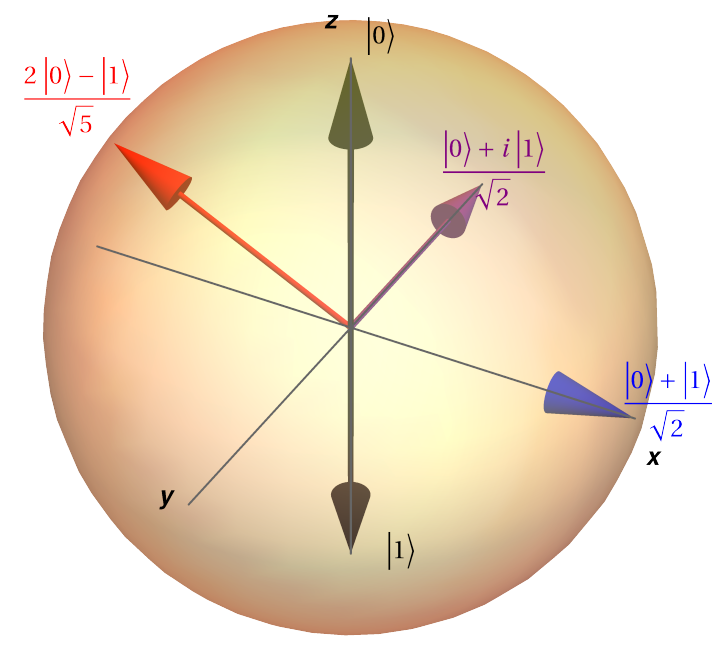
\includegraphics[width=5cm]
        {img-congreso/bloch.png}
    \end{minipage}
    $\stackrel{\E_{xz}\otimes\1 \vspace{1cm}}{\longmapsto}$
    \begin{minipage}{0.4\textwidth}
        \centering
        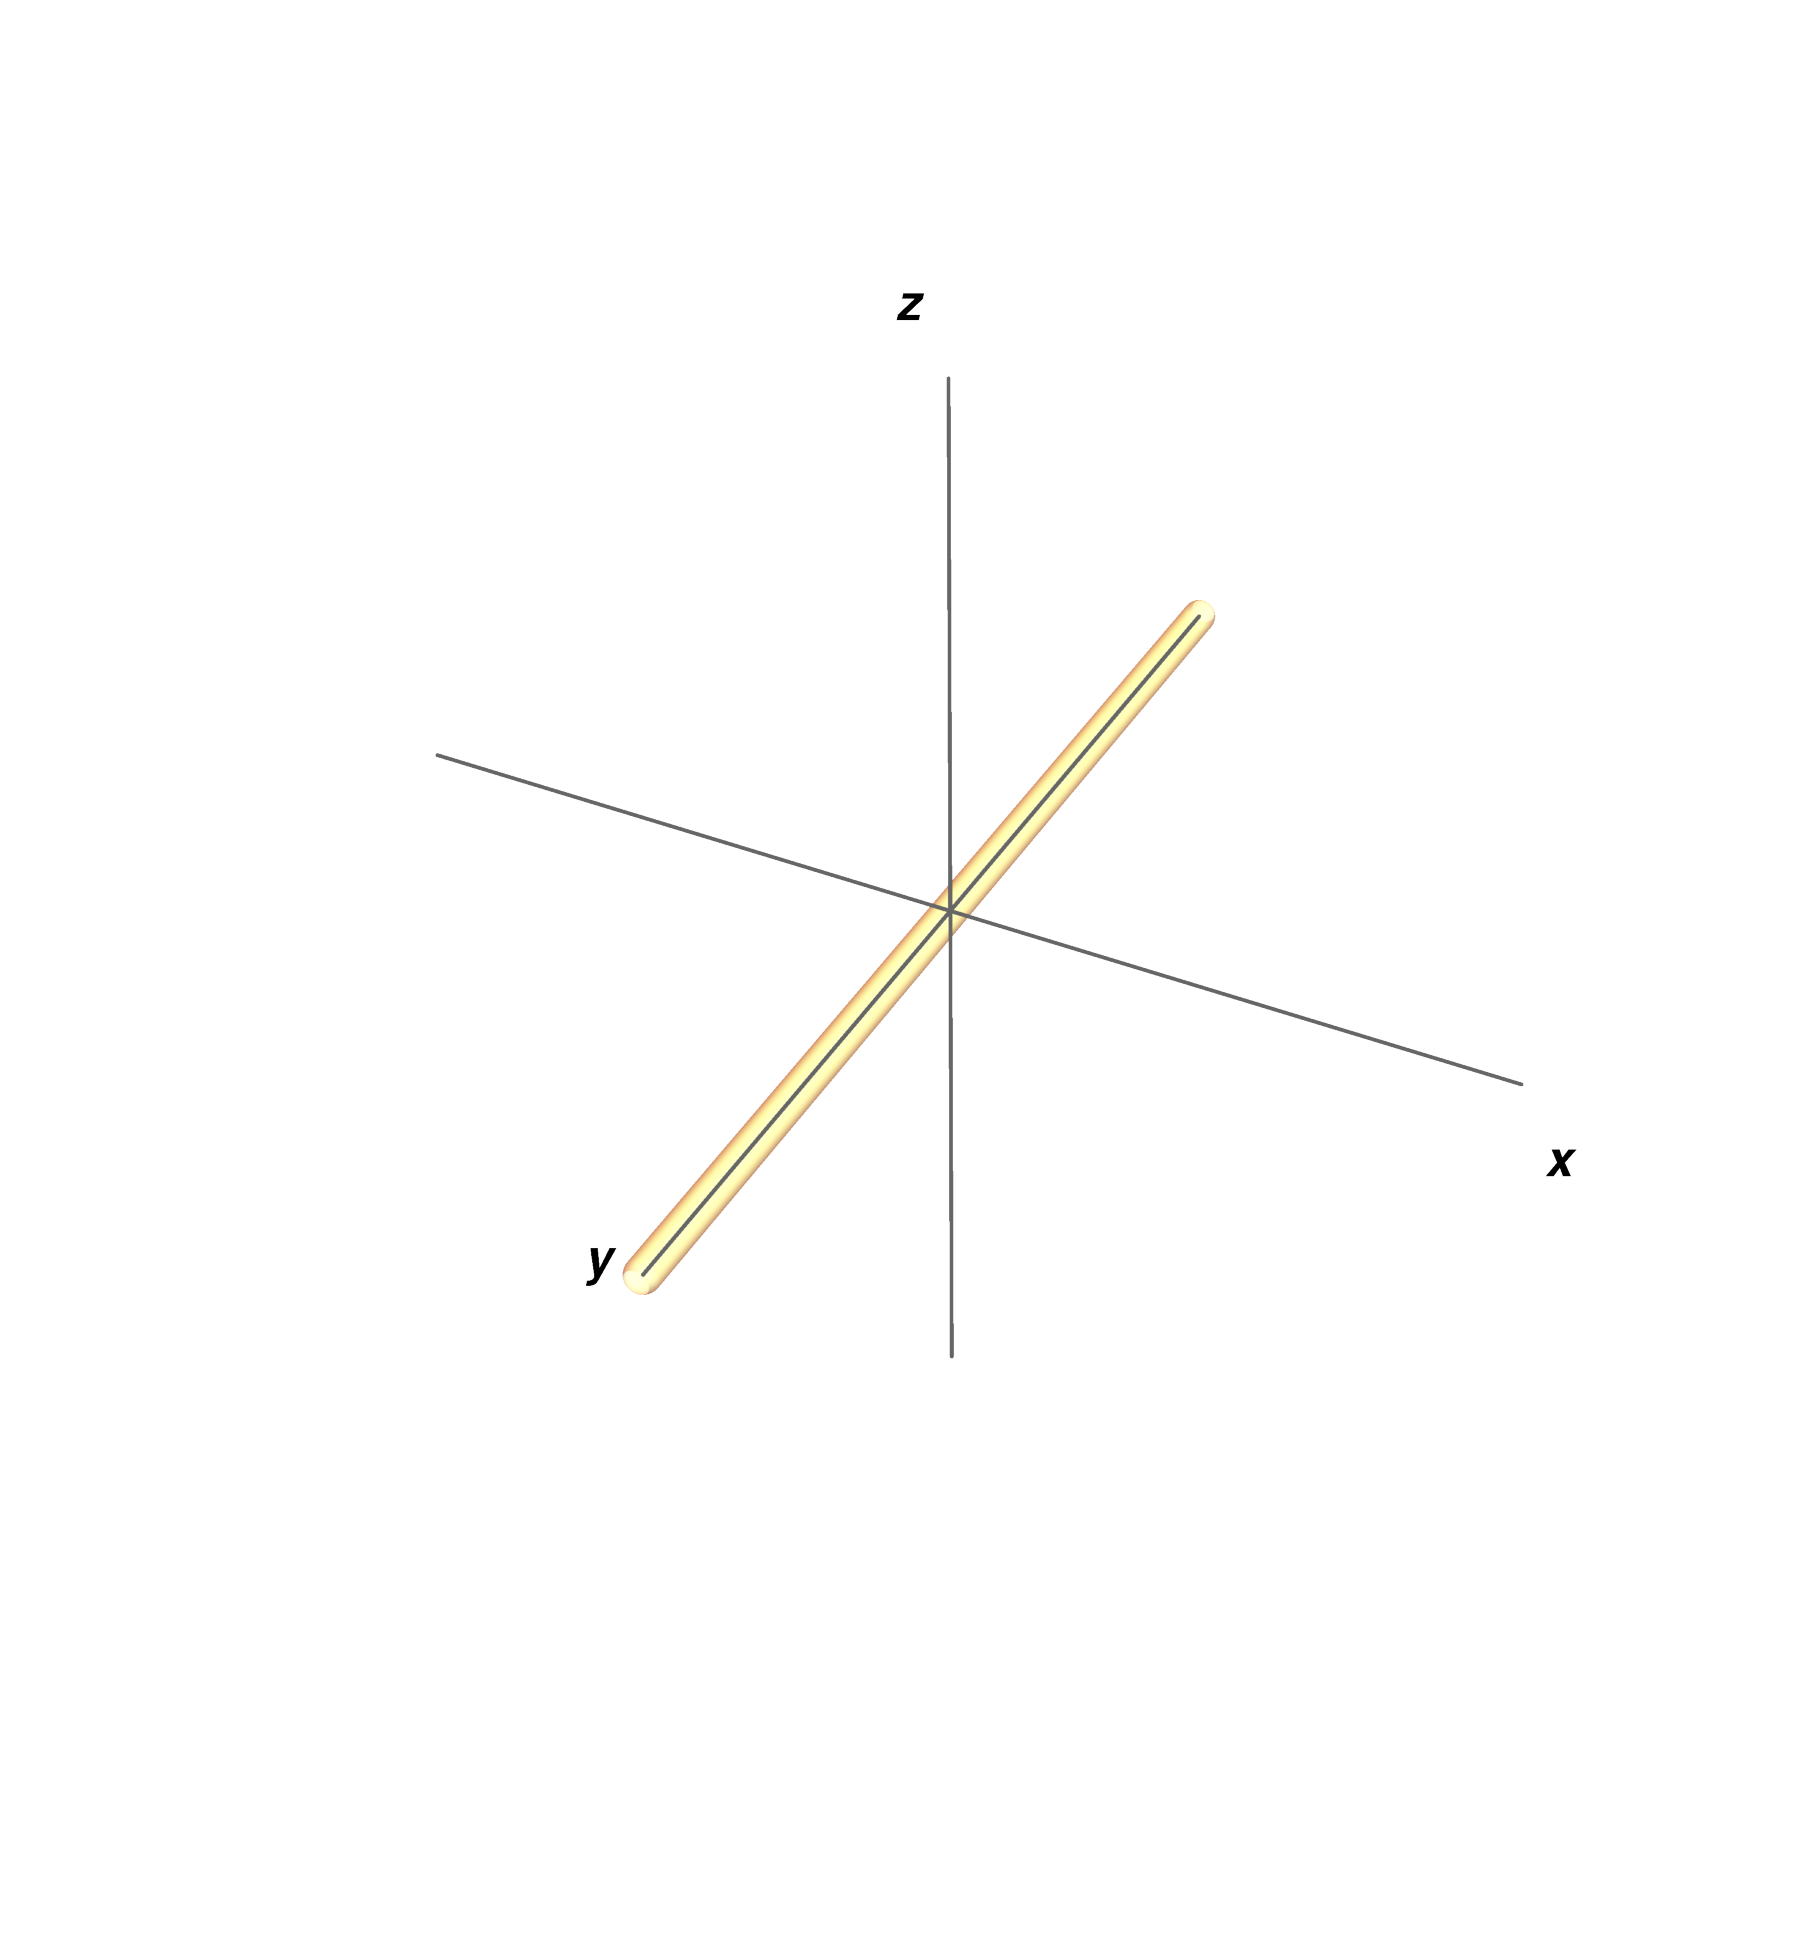
\includegraphics[width=6cm]
        {img-congreso/lineY}
    \end{minipage}
    \caption{Deformación de la esfera de Bloch a un disco sobre el plano $XY$.}
    \label{fig:QC-ex2}
\end{figure} % }}}
Consideremos la operación $\E_{xz}$ que colapsa la esfera de Bloch
al eje $y$, como se muestra en la \Fref{fig:QC-ex2}. El vector de 
Bloch de cualquier punto en la esfera se proyecta hacia el eje $y$.
A partir de la representación geométrica de $\E_{xz}$ 
se puede inferir cómo se transforma el vector $\vec{r}$
de $\rho$ en \eqref{eq:DM-1q}
\begin{align}
\qty(1,r_1,r_2,r_3)\mapsto\qty(1,0,r_2,0),
\label{eq:Bloch-vec-mapToY}
\end{align}
con lo cual se determina $\rho'$ y, seguidamente,
la matriz $\E_{xz}$.
Por lo tanto, la ecuación de transformación de la matriz 
de densidad de 1 qubit, bajo la acción de $\E_{xz}$, es
\begin{align}
\mqty(
\begin{array}{cccc}
\frac{1}{2} & 0 & 0 & \frac{1}{2} \\
0 & \frac{1}{2} & -\frac{1}{2} & 0 \\
0 & -\frac{1}{2} & \frac{1}{2} & 0 \\
\frac{1}{2} & 0 & 0 & \frac{1}{2} \\
\end{array}
)
\frac{1}{2}
\mqty(
1+r_3\\r_1-ir_2\\r_1+ir_2\\1-r_3
)
=
\frac{1}{2}
\mqty(
1\\-ir_2\\ir_2\\1
).
\label{eq:QC-ex2-SR}
\end{align}
Al calcular la matriz de Choi de $\E_{xz}$ notamos 
que $\E_{xz}=\E_{xz}^R$ e, inmediatamente, podemos concluir
que $\E_{xz}$ es completamente positiva. La matriz $\E_{xz}$
es una operación cuántica.

En resumen, en la forma matricial de una operación cuántica $\E$
se considera a $\E$ como una matriz que actúa sobre 
una matriz de densidad vectorizada $\vec{\rho}$. 
Si una operación $\E$ satisface las condiciones de
\eqref{eq:H-condition} a \eqref{eq:positivity-condition}, entonces
es un mapeo afín de matrices de densidad.
Además, el procedimiento de \textit{reshuffle},
establecido en la ecuación \eqref{eq:R-4ind} en notación
de cuatro índices, proporciona una manera para 
calcular la matriz de Choi $D_{\E}$;
y, según el teorema de Choi, si 
$D_{\E}$ es una matriz positiva semidefinida, entonces $\E$ es 
completamente positiva. 
Así, hemos establecido las herramientas y condiciones para evaluar 
si una operación, en su forma matricial, es un canal cuántico.
En la siguiente sección presentaremos la representación de Kraus de las operaciones
cuánticas.

\cpnote{Aca voy}
%}}}
\section{Representación de Kraus} % {{{
% \janote{Reescribí esta sección. El contenido es el mismo, pero debería
% estar escrito de mejor manera.}
% \janote{
% - Enunciar la representación en operadores de suma partiendo de un 
% estado que se acopla con algún entorno
% y llegar a las condiciones para ser CPTP y empezar a conectarlo
% con la sección anterior.} \cpnote{No sabes si hay alguna motivacion que no sea
% con el entorno? Realmente no lo usamos y se me hace meter una complicación adicional}
% \janote{Entonces voy a omitir la motivación con el entorno y en general
%     mencionar al entorno en la explicación.\newline}
% \janote{Introducción\newline}
% \janote{
%     - Invocar el ejemplo del canal de la sección anterior, pero en su 
%     representación de operadores de suma. Aquí quiero hacer la conexión 
%     entre esta y la sección anterior mostrando que los operadores 
%     de Kraus son los eigenvectores de la matriz de Choi.\newline}
% \janote{
%     - Comparar la representacion de suma de operadores y superoperadores
% \newline}

Las operaciones cuánticas también pueden escribirse
en otra representación conocida como la forma de Kraus.
% \cpnote{Cambiar a matricial aca y en todas partes}
% \janote{Hecho.}
La representación recibe su nombre en honor al físico alemán Karl Kraus,
quien en 1971 introdujo esta representación como resultado
del teorema de Stinespring \cite{bengtsson_zyczkowski_2017}.
La representación de Kraus de una operación cuántica es una forma
de reescribir a la ecuación \eqref{eq:E(rho)} como
$\E\qty(\rho)=\sum_k E_k\rho E_k^{\dagger}$,
para algún conjunto de operadores $\{E_k\}$ 
que satisfacen la condición $\sum _kE_k^{\dagger}E_k\leq\1$
\cite{nielsen_chuang_2011}. Esta forma de representar a una
operación cuántica guarda estrecha relación con 
su representación matricial por medio de la matriz de Choi. 
La representación de Kraus de las operaciones cuánticas sólo
es una condición equivalente del teorema de Choi\cpnote{No entiendo eso 
de que una representeacion sea una condición equivalente},
presentado en la sección anterior, sobre los mapeos 
completamente positivos.

En esta sección vamos primero a enunciar la forma canónica
de Kraus y, luego, vamos a mostrar cómo encontrar los 
operadores de Kraus del canal $\E_{xz}$ a partir de la 
matriz de Choi, calculada en el segundo ejemplo de la 
sección anterior.

La representación de Kraus no determina a los operadores
de Kraus de forma única\cpnote{Mal redactado :(}, por lo cual es deseable encontrar
una forma canónica. Un conjunto de operadores de Kraus 
canónicos se puede obtener a partir de los eigenvectores,
reordenados como matrices, de la matriz de Choi de la 
operación cuántica \cite{bengtsson_zyczkowski_2017}.
Además, la raíz cuadrada de los eigenvalores de la 
matriz de Choi proporcionan los pesos de los operadores
de Kraus en su forma canónica.  

\textbf{Forma canónica de Kraus.} Un mapeo completamente 
positivo $\E:\mathcal{M}^{(N)}\to\mathcal{M}^{(N)}$ se
puede escribir como
\begin{align}
\rho \longrightarrow \rho' = 
\sum_{k=1}^{r\leq N^2}d_k\chi_k\rho\chi_k^{\dagger}
= \sum_{i=1}^rE_k\rho E_k^{\dagger},
\label{eq:Kraus-canonical}
\end{align}
donde $r$ es el rango de la matriz de Choi y $d_k$ y $\chi_k$ 
\cpnote{Estoy confundido. Si chi son vectores, y haces chi rho chi, te queda un 
escalar? O como loe haces?}
son sus eigenvalores y eigenvectores normalizados, respectivamente; 
adicionalmente, los operadores $E_k$ deben satisfacer la condición
\begin{align}
  \Tr\qty(E_k^{\dagger}E_k)=d_i\delta_{ij}.
  \label{eq:Tr-Kraus-canonical}
\end{align}
Si $\E$ preserva la 
traza de $\rho$, entonces
\begin{align}
  \sum_kE_k^{\dagger}E_k=\1
  &&\Rightarrow&&
  \sum_{k=1}^rd_k=N .
  \label{eq:completeness-Kraus-canonical}
\end{align}
Se conoce como rango de Kraus al número de operadores 
en la forma canónica y es igual al rango de la matriz de Choi $r$
\cite{bengtsson_zyczkowski_2017}.

Ahora, con la forma canónica de Kraus introducida podemos
discutir un ejemplo de cómo calcular la representación de Kraus
de una operación cuántica.
La matriz de Choi de $\E_{xz}$ es igual a  su representación
matricial en \eqref{eq:QC-ex2-SR}.
Para encontrar la representación canónica de Kraus de $\E_{xz}\qty(\rho)$
vamos a diagonalizar a $D_{\E_{xz}}$ $(D_{\E_{xz}}=\E_{xz})$
para encontrar
sus eigenvalores y eigenvectores; luego, al reordenar
cada eigenvector como matriz y multiplicarlo por la raíz cuadrada
del eigenvalor correspondiente obtendremos los operadores 
de Kraus $E_k$ de $\E_{xz}$. Finalmente, al operar los $E_k$ 
con la matriz de densidad de 1 qubit, siguiendo la forma de 
Kraus en \eqref{eq:Kraus-canonical}, mostraremos que se obtiene el 
mismo resultado $\rho'$ en \eqref{eq:QC-ex2-SR}.

Al calcular con los eigenvectores $\ket{\chi_k}$ de $D_{\E_{xz}}$ \cpnote{redaccion} se obtiene
\begin{align}
\begin{tabular}{lcl}
$\ket{\chi_1}=\frac{1}{\sqrt{2}}\qty(\ket{00}+\ket{11})$, & \hspace{1cm}
& $ \ket{\chi_{2}}=\frac{1}{\sqrt{2}}\qty(-\ket{01}+\ket{10})$, \\
$\ket{\chi_{3}}=\frac{1}{\sqrt{2}}\qty(-\ket{00}+\ket{11})$, & \hspace{1cm}
& $\ket{\chi_4}=\frac{1}{\sqrt{2}}\qty(\ket{01}+\ket{10})$,
\end{tabular}
\end{align}
cuyos respectivos eigenvalores son $d_1=1,d_2=1,d_3=0,d_4=0$. 
Se reordenan cada uno de los $\ket{\chi_k}$ en una matriz
de $2\times2$, siguiendo el proceso inverso de vectorización
en \eqref{eq:matrix-to-vector}, y se multiplica por $\sqrt{d_k}$ 
para obtener los operadores de Kraus canónicos $E_k$; así se obtienen
\begin{align}
E_1&=
\frac{1}{\sqrt{2}}
\mqty(
1 & 0\\
0 & 1
),
&
E_2&=
\frac{1}{\sqrt{2}}
\mqty(
0 & -1\\
1 & 0
),
\end{align}
y $E_3=E_4=0$, dado que $d_3=d_4=0$. 
Finalmente, escribimos a $\E_{xz}\qty(\rho)$ en su representación 
de Kraus para revisar que se obtiene la misma matriz
de densidad $\rho'$ obtenida en la sección anterior,
\begin{align}
\rho'=&
\frac{1}{2}
\mqty(
1 & 0\\
0 & 1
)
\mqty(
\frac{1+r_3}{2}& \frac{r_1-ir_2}{2}\\
\frac{r_1+ir_2}{2} & \frac{1-r_3}{2}
)
\mqty(
1 & 0\\
0 & 1
)^{\dagger}
+
\frac{1}{2}
\mqty(
0 & -1\\
1 & 0
)
\mqty(
\frac{1+r_3}{2}& \frac{r_1-ir_2}{2}\\
\frac{r_1+ir_2}{2} & \frac{1-r_3}{2}
)
\mqty(
0 & 1\\
-1 & 0
)^{\dagger}&
\nonumber\\
\rho'=&
\frac{1}{2}
\mqty(
1 & -ir_2\\
ir_2 & 1
).
\label{eq:QC-ex2-KR}
\end{align}
En efecto se obtiene el mismo resultado $\rho'$ que 
en  \eqref{eq:QC-ex2-SR}, pero reordenada como una matriz. 

%Los eigenvectores de la matriz de Choi de una operación cuántica $\E$,
%reordenados como matrices, se
%reciben el nombre de operadores de Kraus $E_i$ de la operación cuántica.
%Los operadores $E_i$ linealmente independientes  
%pueden ser hasta $N^2$ \cite{nielsen_chuang_2011}, igual a la dimensión 
%del espacio de los operadores lineales que actúan sobre un espacio de
%Hilbert de dimensión $N$. 
%Finalmente, una operación cuántica $\E$ preserva la traza de la matriz de densidad 
%si y sólo sus operadores de Kraus $E_i$ satisfacen la condición
%\cite{bengtsson_zyczkowski_2017}
%\begin{align}
%\sum_iE_i^{\dagger}E_i=\1.
%\label{eq:kraus-tp-cond}
%\end{align}

En resumen, las ecuaciones \eqref{eq:Kraus-canonical},
\eqref{eq:Tr-Kraus-canonical} y \eqref{eq:completeness-Kraus-canonical}
caracterizan la representación de Kraus canónica de un canal cuántico. 
Hasta aquí hemos presentado dos formas distintas de representar a un 
canal cuántico: (1) la forma matricial, una matriz cuadrada
de tamaño $N^2$ que actúa sobre una matriz de densidad vectorizada 
con $N^2$ entradas; y (2) la representación de Kraus, operadores 
que pertenecen al espacio de los operadores lineales que 
actúan sobre el espacio de Hilbert del sistema actuando 
sobre la matriz de densidad. La matriz de Choi
proporciona una manera de conectar ambas 
representaciones. Por un lado, si $D_{\E}$ es la matriz de 
Choi de un canal cuántico $\E$, entonces $D_{\E}^R$ es 
la representación matricial de $\E$;
por otro lado, los eigenvectores de $D_{\E}$, reordenados
como matrices y multiplicados por la raíz cuadrada de sus eigenvalores 
correspondientes, dan como resultado los operadores de Kraus 
canónicos $E_k$ de $\E$. Ahora que contamos con dos 
formas de representar a una operación cuántica
será útil revisar algunos ejemplos de canales cuánticos
de 1 qubit en la siguiente sección.

%}}}
\section{Canales cuánticos de 1 qubit} \label{sec:CC's-1q-ejemplos}
% {{{
\cpnote{Aca voy}

\janote{
- Hablar de que se gana intuición pensando en la acción de un canal de 1
qubit como la manera en que deforma la esfera de Bloch\newline}
\janote{
- Ejemplos: phase-flip channel, depolarizing y amplitude damping\newline}

Los canales cuánticos de 1 qubit proporcionan buena intuición 
para completar el marco teórico de las operaciones cuánticas. 
La ventaja particular que tienen estos canales cuánticos 
es que es posible visualizar geométricamente la acción de
la operación sobre la esfera de Bloch. 
En esta sección vamos a presentar tres canales cuánticos 
representativos del caso de un 1 qubit. Vamos a presentar 
la forma matricial y la representación de Kraus de 
cada uno de los canales.

\subsection{Canal inversor de fase y bit}
El canal inversor de fase y bit $\E_{BPF}$ transforma 
con probabilidad $1-p$ a un estado de 1 qubit de la forma  
\begin{align}
   \ket{\psi}=e^{i\gamma}\qty[\cos\qty(\frac{\theta}{2})\ket{0}
  +e^{i\phi}\sin \qty(\frac{\theta}{2})\ket{1}],
   \label{eq:psi-1qubit}
 \end{align} 
con $\ket{0}$ y $\ket{1}$ los eigenestados de 
la matriz de Pauli $\sigma_z$, según las transformaciones 
$\theta\to\theta+\pi$ y $\phi\to\phi+2\pi$ 
\cite{nielsen_chuang_2011}. 
Si consideramos a la matriz de densidad de 1 qubit
$\rho^1$ en \eqref{eq:DM-1q} el canal $\E_{BPF}$ 
transforma  al vector $\vec{r}$ como \cite{nielsen_chuang_2011}
\begin{align}
\qty(1,r_1,r_2,r_3)\rightarrow&\Big(1,\qty(1-2p)r_1,r_2,\qty(1-2p)r_3\Big).
\label{eq:bit-phase-flip-Bloch-trans}
\end{align}
Geométricamente, el vector de Bloch $\qty(r_1,r_2,r_3)$ es 
proyectado al eje $y$ y las componentes 
en $x$ y $z$ son atenuadas, como se muestra en la 
\Fref{fig:bit-phase-flip}.
Notemos que el canal cuántico $\E_{xz}$, discutido 
en la sección 2.2 y 2.3, es un caso particular de $\E_{BPF}$ $(p=0.5)$.

\begin{figure}
\centering
\begin{minipage}{.4\textwidth}
    \centering
    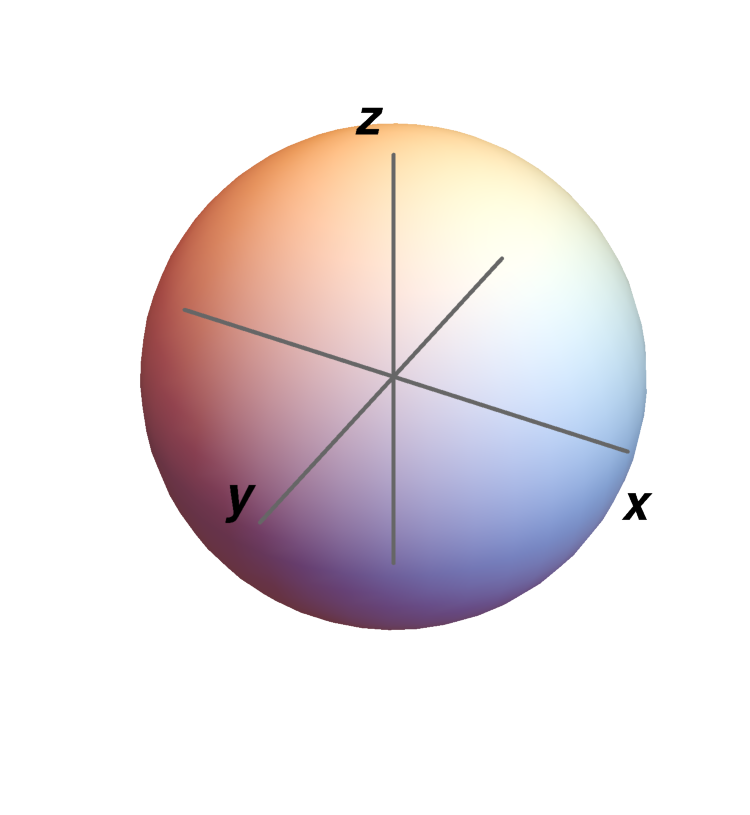
\includegraphics[width=6cm]{images/bloch-ball}
\end{minipage}
$\longmapsto$
\begin{minipage}{0.4\textwidth}
    \centering
    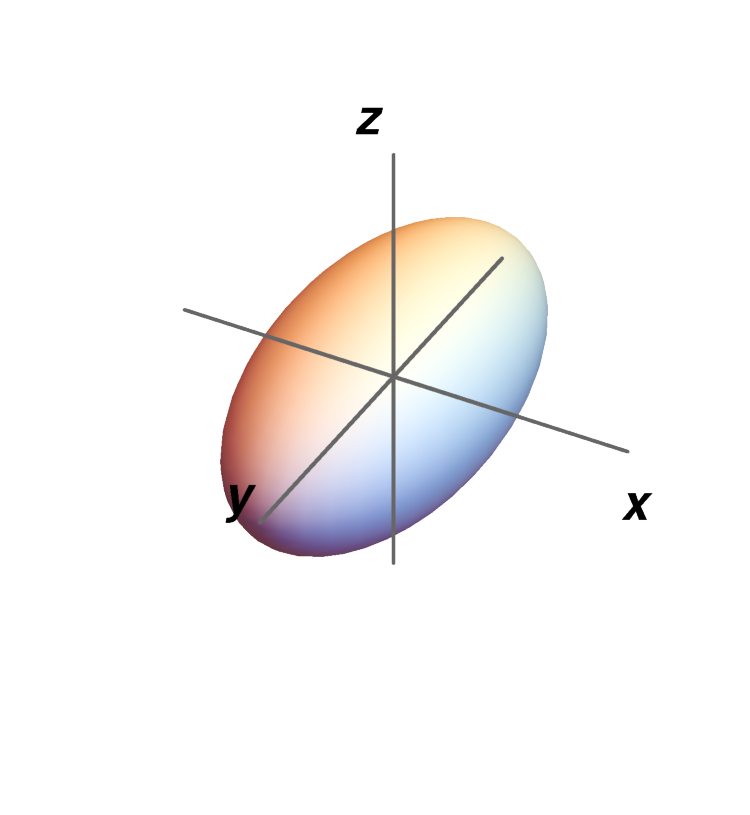
\includegraphics[width=6cm]{images/bit-phase-flip}
\end{minipage}
\caption{Efecto del canal inversor de fase y bit sobre la esfera de Bloch, 
para $p=0.3$.}
\label{fig:bit-phase-flip}
\end{figure}
Con ayuda de \eqref{eq:bit-phase-flip-Bloch-trans} y la matriz
de densidad de 1 qubit en \eqref{eq:DM-1q} 
escrita en la base canónica podemos calcular 
$\rho$ y $\E_{BPF}\qty(\rho)$. Se vectorizan a $\rho$ y 
$\E_{BPF}\qty(\rho)$ para luego calcular la forma matricial 
de $\E_{BPF}$ con métodos elementales de álgebra lineal.
Así se obtiene que la ecuación $\E_{BPF}(\rho)=\rho'$ 
en su forma matricial es
\begin{align}
\frac{1}{2}
\mqty(
1-p & 0 & 0 & p \\
0 & 1-p & -p & 0 \\
0 & -p & 1-p & 0 \\
p & 0 & 0 & 1-p \\
)
\frac{1}{2}
\mqty(
1+r_3\\r_1-ir_2\\r_1+ir_2\\1-r_3
)
=
\frac{1}{2}
\mqty(
1+\qty(1-2p)r_3\\
\qty(1-2p)r_1-i r_2\\
\qty(1-2p)r_1+i r_2\\
1-\qty(1-2p)r_3
).
\label{eq:bpf-supero}
\end{align}
Para encontrar los operadores de Kraus se calculan los eigenvectores
y eigenvalores de $D_{\E_{BPF}}$. Para~ello, calculamos antes
$D_{\E_{BPF}}$ aplicando procedimiento de \textit{reshuffle}
\begin{align}
  D_{\E_{BPF}}=\E_{BPF}^R=
  \mqty(
	 1-p & 0 & 0 & 1-p \\
	 0 & p & -p & 0 \\
	 0 & -p & p & 0 \\
	 1-p & 0 & 0 & 1-p
  ).
  \label{eq:Choi-E_bpf}
\end{align}
Los eigenvectores normalizados de $D_{\E_{BPF}}$, 
reordenados como matrices y multiplicados por 
la raíz cuadrada de sus eigenvalores respectivos, son
\begin{align}
E_1&=
\sqrt{p}
\mqty(
1 & 0\\
0 & 1
)&
E_2&=
\sqrt{1-p}
\mqty(
0 & -1\\
1 & 0
),
&E_3=E_4=0.
\label{eq:bpf-kraus}
\end{align}
Así, hemos encontrado la forma matricial y de Kraus del canal
cuántico inversor de fase y bit $\E_{BPF}$. Se puede evaluar directamente que 
tanto la matriz en \eqref{eq:bpf-supero} como los operadores $E_i$
en \eqref{eq:bpf-kraus} cumplen con las condiciones respectivas
para ser canales cuánticos.

\subsection{Canal depolarizante}
El canal depolarizante $\E_{Dep}$ 
atenúa todas las coordenadas 
del vector de Bloch con probabilidad $1-p$, como se muestra
en la \Fref{fig:depolarizing}. Por consiguiente, 
se sigue que el vector $\vec{r}$ de la matriz 
de densidad de 1 qubit se transforma como \cite{nielsen_chuang_2011}
\begin{align}
\qty(1,r_1,r_2,r_3)\rightarrow&\Big(1,\qty(1-p)r_1,\qty(1-p)r_2,\qty(1-p)r_3\Big).
\label{eq:depolarizing-bloch-vec}
\end{align}

Cuando $p=1$ el canal mapea todos los estados 
de 1 qubit al estado de máxima ignorancia $\1/2$, 
o también conocido como el estado máximamente mixto 
\cite{bengtsson_zyczkowski_2017}. Geométricamente, 
la esfera de Bloch se deforma a un punto en el origen.
\begin{figure}
    \centering
    \begin{minipage}{.4\textwidth}
        \centering
        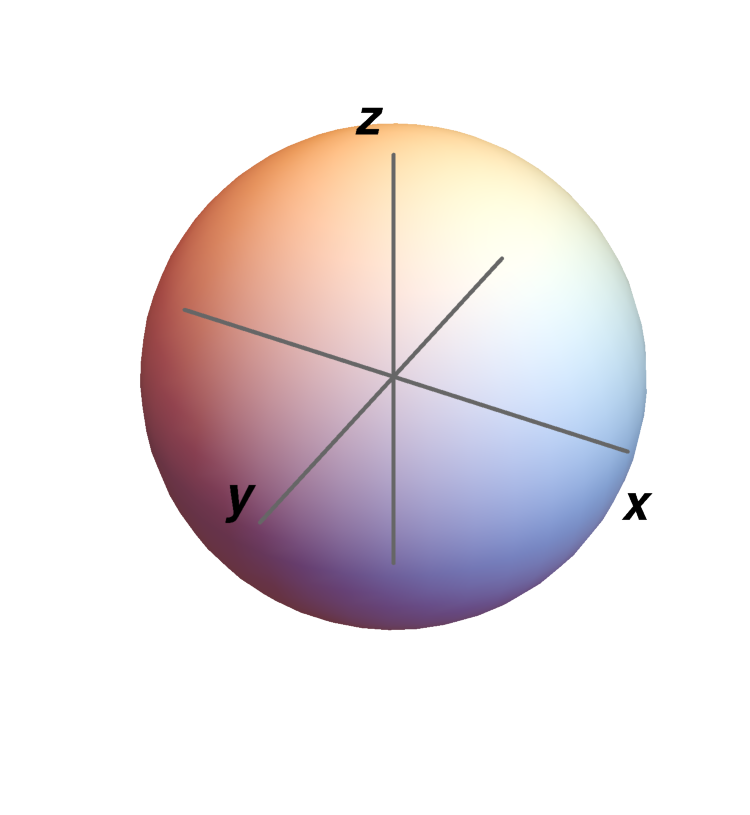
\includegraphics[width=6cm]{images/bloch-ball}
    \end{minipage}
    $\longmapsto$
    \begin{minipage}{0.4\textwidth}
        \centering
        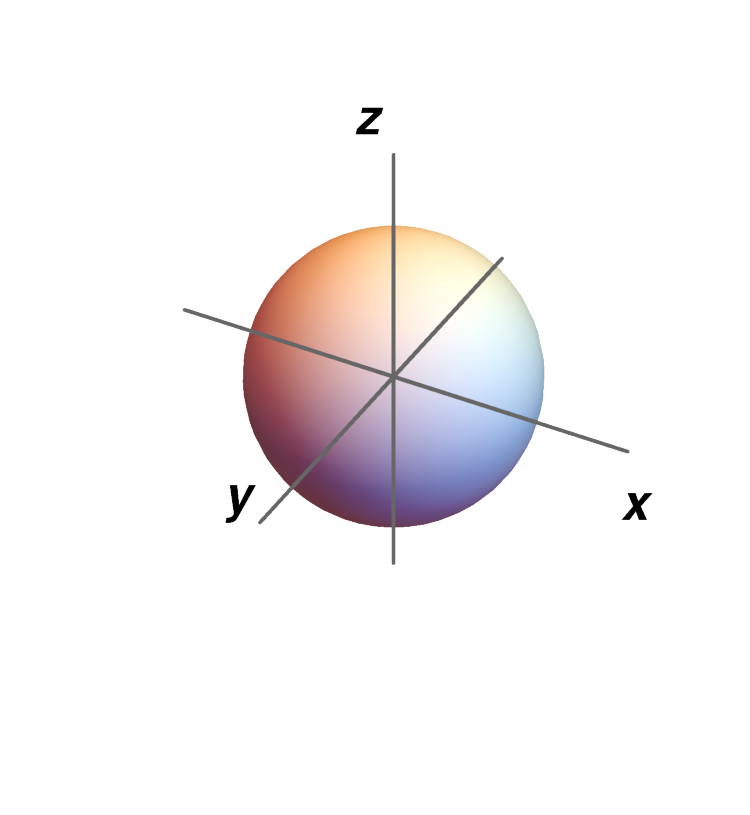
\includegraphics[width=6cm]{images/depolarizing}
    \end{minipage}
    \caption{Efecto del canal depolarizante sobre la esfera de Bloch, 
    para $p=0.4$.}
    \label{fig:depolarizing}
\end{figure}

Se repite el procedimiento del ejemplo anterior para calcular 
la representación matricial de $\E_{Dep}$ y asi se obtiene
que la ecuación $\E_{Dep}(\rho)=\rho'$ en su forma matricial es
\begin{align}
\mqty(
1-\frac{p}{2} & 0 & 0 & \frac{p}{2} \\
0 & 1-p & 0 & 0 \\
0 & 0 & 1-p & 0 \\
\frac{p}{2} & 0 & 0 & 1-\frac{p}{2}
)
\frac{1}{2}
\mqty(
1+r_3\\r_1-ir_2\\r_1+ir_2\\1-r_3
)
=
\frac{1}{2}
\mqty(
1+\qty(1-p)z\\
\qty(1-p)\qty(x-i y)\\
\qty(1-p)\qty(x+i y)\\
1-\qty(1-p)z
).
\end{align}
Se aplica el procedimiento de \textit{reshuffle}
para determinar a la matriz de Choi
\begin{align}
D_{\E_{Dep}}=
\mqty(
 1-\frac{p}{2} & 0 & 0 & 1-p \\
 0 & \frac{p}{2} & 0 & 0 \\
 0 & 0 & \frac{p}{2} & 0 \\
 1-p & 0 & 0 & 1-\frac{p}{2} 
).
\label{•}
\end{align}
Ahora, con $D_{\E_{Dep}}$ se calculan sus 
eigenvectores y eigenvalores para encontrar la forma 
canónica de Kraus, siguiendo lo establecido en la
sección 2.3. Se encuentran los operadores de Kraus
canónicos:
\begin{align}
E_0&=
\sqrt{1-\frac{3p}{4}}
\mqty(
1 & 0\\
0 & 1
),&
E_1&=
\frac{\sqrt{p}}{2}
\mqty(
-1 & 0\\
0 & 1
),\\
E_2&=
\frac{\sqrt{p}}{2}
\mqty(
0 & -1\\
1 & 0
), &
E_3&=
\frac{\sqrt{p}}{2}
\mqty(
0 & 1\\
1 & 0
).
\end{align}

Notemos que los canales de inersión de fase y bit y el
depolarizante dejan invariante al estado máximamente mixto
$\rho=\1/2$. Esto se puede visualizar fácilmente en la representación
de Bloch, pues dejar invariante a $\rho=\1/2$ significa dejar 
invariante al origen de coordenadas. Todos los canales 
cuánticos que satisfacen $\E(\1/2)=\1/2$
se conocen como canales unitales. 
A continuación, el último ejemplo que vamos a presentar
es el de un canal que no satisface la condición de unitalidad.

\subsection{Canal de amortiguamiento de amplitud}
La acción del canal de amortiguamiento de amplitud $\E_{AF}$
sobre la esfera de Bloch es tal que la deforma a un elipsoide
cuyo centro geométrico no es el origen de coordenadas, 
como se muestra en la \Fref{fig:amp-damp}. 
El canal $\E_{AF}$ transforma al vector $\vec{r}$ de 
la matriz de densidad de 1 qubit como
\cite{nielsen_chuang_2011}
\begin{align}
\qty(1,r_1,r_2,r_3)\rightarrow&\Big(1,r_1\sqrt{1-\gamma},
r_2\sqrt{1-\gamma},\gamma+\qty(1-\gamma)r_3\Big).
\label{eq:damp-phase}
\end{align}
\begin{figure}
    \centering
    \begin{minipage}{.4\textwidth}
        \centering
        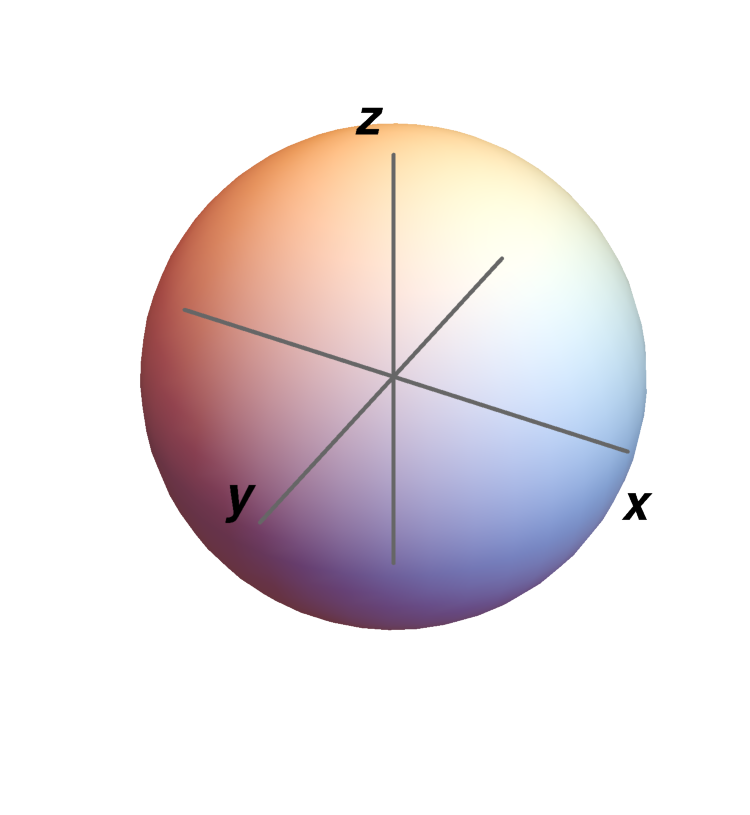
\includegraphics[width=6cm]{images/bloch-ball}
    \end{minipage}
    $\longmapsto$
    \begin{minipage}{0.4\textwidth}
        \centering
        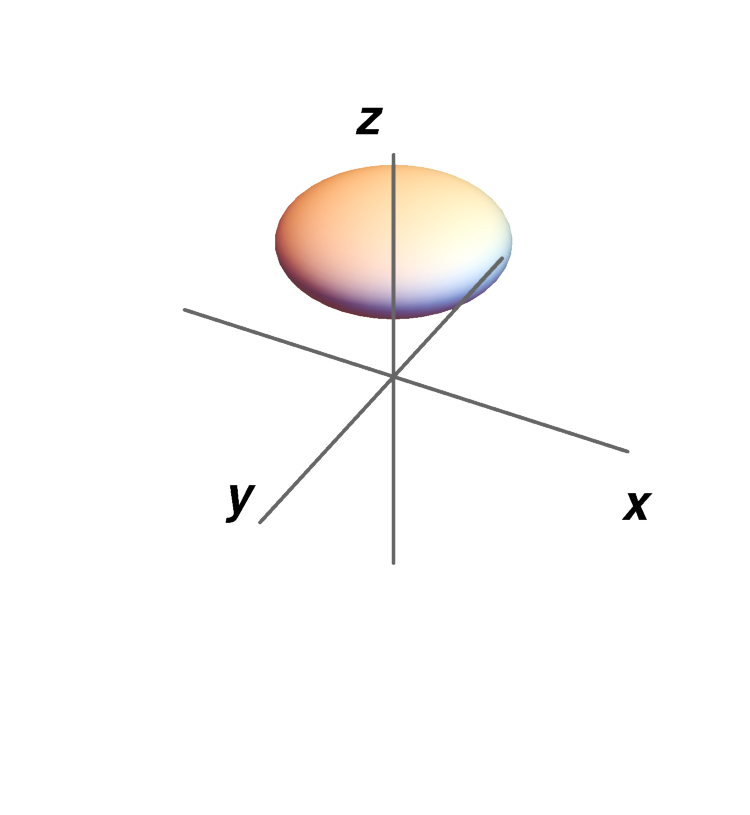
\includegraphics[width=6.2cm]{images/gen-amplitude-damping}
    \end{minipage}
    \caption{Efecto del canal generalizado de amortiguamiento de 
        amplitud sobre la esfera de Bloch, 
        para $p=0.4$.}
    \label{fig:amp-damp}
\end{figure}
Con la transformación de $\vec{r}$ determinada se repite 
el mismo procedimiento de los ejemplos anteriores 
para calcular la representación matricial de $\E_{AF}$. 
Por tanto, la ecuación $\E_{AF}(\rho)=\rho'$, escrita 
en forma matricial, es 
\begin{align}
\mqty(
 1 & 0 & 0 & \gamma  \\
 0 & \sqrt{1-\gamma } & 0 & 0 \\
 0 & 0 & \sqrt{1-\gamma } & 0 \\
 0 & 0 & 0 & 1-\gamma  
)
\frac{1}{2}
\mqty(
1+r_3\\r_1-ir_2\\r_1+ir_2\\1-r_3
)
=
\frac{1}{2}
\mqty(
1+\gamma+\qty(1-\gamma)z\\
\sqrt{1-\gamma}\qty(x-i y)\\
\sqrt{1-p}\qty(x+i y)\\
1-\gamma-\qty(1-\gamma)z
).
\label{eq:damp-ph-matrix}
\end{align}
Se calcula la matriz de Choi de $\E_{AF}$ con la transformación
de \textit{reshuffle} a la matriz en \eqref{eq:damp-ph-matrix}
y se~obtiene
\begin{align}
D_{\E_{AF}}=
\mqty(
 1 & 0 & 0 & \sqrt{1-\gamma } \\
 0 & \gamma  & 0 & 0 \\
 0 & 0 & 0 & 0 \\
 \sqrt{1-\gamma } & 0 & 0 & 1-\gamma  
).
\end{align}
Se calculan los eigenvectores normalizados de $D_{\E_{AF}}$, multipicados
por la raíz cuadrada de sus eigenvalores asociados, y se reordenan
como matrices. Así, se obtienen los operadores de Kraus 
del canal de amortiguamiento de amplitud:
\begin{align}
E_1&=
\sqrt{1-\gamma }
\mqty(
\frac{1}{\sqrt{1-\gamma }} & 0 \\
0 & 1
),&
E_2&=
\sqrt{\gamma }
\mqty(
0 & 1 \\
0 & 0 
),
&
E_3=E_4=0.
\end{align}

Para resumir, hemos expuesto 3 ejemplos de canales cuánticos de 1 qubit:
el canal de inversión de fase y bit, el canal depolarizante 
y el canal de amortiguamiento
de amplitud. La acción de los canales cuánticos de 1 qubit 
es más sencilla de visualizar en la representación de la esfera de Bloch
y su deformación bajo la acción del canal. 
El canal de inversión de fase y bit deforma la
esfera de Bloch de tal forma que encoge las componentes $x$ y $z$ en 
un factor $1-2p$, y deja invariante la componente
$y$ de cada punto en la esfera, con $p$ un parámetro que indica la
probabilidad de ocurrir la acción del canal. 
El canal depolarizante 
atenúa todas las componentes del vector de Bloch de manera uniforme
en un factor $1-p$; la esfera de Bloch se encoge
continuamente hasta un punto en el origen. Finalmente, 
el canal de amortiguamiento de amplitud deforma la esfera de Bloch
a un elipsoide cuyo centro geométrico no coincide con el origen, por
ello, se dice que el canal no es unital; son canales unitales aquellos 
que dejan invariante al estado máximamente mixto, 
que en la esfera de Bloch es el origen de coordenadas.

El formalismo de los canales cuánticos proporciona un marco 
teórico para describir el cambio dinámico de los estados cuánticos 
de sistemas abiertos. Un nombre más descriptivo para 
los canales cuánticos es mapeos completamente 
positivos que preservan la traza \cite{bengtsson_zyczkowski_2017},
para enfatizar que los canales cuánticos son mapeos afines de matrices de 
densidad, que transforman estados positivos en estados positivos,
aún cuando el sistema se acopla con un sistema secundario y el estado
total es uno entrelazado. 
Dos formas de representar a los canales cuánticos
se presentaron en este capítulo, la forma matricial y 
la representación de Kraus, cuya conexión entre ambas representaciones
es posible mediante la matriz de Choi.
La preferencia por alguna representación u otra está determinada 
por la naturaleza del problema a resolver. 
% }}}
